\section{Auswertung}
\label{sec:Auswertung}
\subsection{Volumen und Dichte}
\label{sec:Vol und Dich}
Zuerst werden die Mittelwerte aus den gemessenen Werte des Durchmesser der kleineren und der größeren Kugel bestimmt.
\begin{align}
d_\mathrm{kl}&=(1,546\pm0.007)\si{\centi\meter}\\
d_\mathrm{gr}&=(1,561\pm0.006)\si{\centi\meter}
\end{align}
Dadurch lässt sich nun das Volumen der beiden Kugel mit Hilfe der Formel \eqref{eqn:vol}
berechnen:
\begin{align}
V_{\mathrm{Kugel}}&=\frac{4}{3}\pi \left(\frac{d_{\mathrm{Kugel}}}{2}\right)^3\label{eqn:vol}\\
\intertext{Für die kleinere Kugel ergibt sich dann}\\
V_{\mathrm{kl}}&=(1,935\pm0,026)\si{\cubic\centi\meter}\\
\intertext{und für die größere Kugel}\\
V_\mathrm{gr}&=(1,991\pm0,023)\si{\cubic\centi\meter}\\
\end{align}
Durch das Volumen und die gemessenen Massen der Kugeln kann nun die Dichten der Kugeln mit der Formel \eqref{eqn:rho}
bestimmt werden.
\begin{align}
\rho_{\mathrm{Kugel}}&=\frac{m}{V}\label{eqn:rho}\\
\intertext{Masse der Kugeln:}\\
m_{\mathrm{kl}}&=4,46\si{\gram}\\
m_{\mathrm{gr}}&=4,96\si{\gram}\\
\intertext{Daraus ergeben sich die folgenden Dichten}\\
\rho_{\mathrm{kl}}&=(2,305\pm0,031)\si{\gram\per\cubic\centi\meter}\\
\rho_{\mathrm{gr}}&=(2,492\pm0,029)\si{\gram\per\cubic\centi\meter}
\end{align}
\subsection{Berechnung der Apparatekonstante}
Nun wird die Apparatekontante für die größere Kugel $\mathrm{K}_{\mathrm{gr}}$ aus
der Formel \eqref{eqn:vis} berechnet. Dafür werden erst die gemessenen Zeiten aus der Tabelle \ref{tab:kg}
gemittelt.
\begin{table}
  \centering
  \caption{Zeiten der Kugeln bei $294,15\si{\kelvin}$.}
  \label{tab:kg}
  \begin{tabular}{c c}
  \toprule
  $t_{\mathrm{kl}}/\si{\second}$ & $t_{\mathrm{gr}}/\si{\second}$ \\
bei einer Strecke von $10\si{\centi\meter}$ & bei einer Strecke von $5\si{\centi\meter}$\\
\midrule
12,44   & 41,41\\
12,36   & 41,13\\
12,59  	& 41,62\\
13,10   & 41,93\\
12,63   & 41,25\\
12,21   & 42,29\\
12,56   & 41,30\\
12,69   & 41,89\\
12,69   & 41,10\\
12,44   & 42,00\\
\bottomrule
  \end{tabular}
\end{table}

Für gemittelten Werte ergibt sich:
\begin{align}
\overline{t}_{\mathrm{kl}} &= (12,57\pm0,23)\si{\second}\\
\overline{t}_{\mathrm{gr}} &= (41,59\pm0,39)\si{\second}\\
\intertext{Da die größere Kugel bei der Messung nur $5\si{\centi\meter}$
zurrücklegt, muss die Zeit verdoppelt werden, damit sich
die Apparatekonstante $\mathrm{K}_{\mathrm{gr}}$ auch auf $10\si{\centi\meter}$ bezieht.
Dies ist notwendig, damit diese für weitere Rechnungen benutzet werden kann. Folglich wird  }\\
\overline{t}_{\mathrm{gr}} &= (83,18\pm0,78)\si{\second}\\
\intertext{verwendet. Da die Apparatekonstante}\\
 K_{\mathrm{kl}}&=0,07640\si{\milli\pascal\cubic\centi\meter\per\gram}\\
\end{align}
gegebene ist, lässt sich die Viskosität durch einsetzen der gemessenen Werte der kleineren Kugel in die Formel \ref{eqn:vis} berechen.
Für die Viskosität ergibt somit sich:
\begin{align}
  \eta&=(1,26\pm0,04)\si{\milli\pascal\second}.\\
\intertext{Wird die Formel \eqref{eqn:vis} nun nach der Apparatekostante umgestellt, ergibt sich}\\
\mathrm{K}&=\frac{\eta}{\left( \rho_{\mathrm{K}}-\rho_{\mathrm{Fl}}\right)\cdot t}\label{eqn:k}
\intertext{Durch die Formel \eqref{eqn:k} lässt sich nun $\mathrm{K}_{\mathrm{gr}}$ bestimmen, indem nun die berechnete Viskosität, Dichte der
größeren Kugel und ihrer gemittelten Zeit in die Gleichung einsetzt werden.}\\
\mathrm{K}_{\mathrm{gr}}&=(10.1\pm0.4)\si{\micro\pascal\cubic\centi\meter\per\gram}
\end{align}
\subsection{Viskosität bei Temperaturänderung}
Die gemittelten Zeiten für die unterschiedlichen Temperaturen die in der Tabelle \ref{tab:temp}
zusehen sind wurden nur mit der großen Kugel gemessen. Bei der Berechnung der Viskositäten
wurde angenommen, dass die Dichte des Wassers bei unterschiedlichen Temperaturen ungefähr konstant bleib.
\begin{table}
   \centering
   \caption{gemittelte Zeiten für eine Strecke von $10\si{\centi\meter}$ bei unterschiedlichen Temperaturen und die sich daraus aus Formel \eqref{eqn:vis} ergebenen Viskositäten.}
   \label{tab:temp}
   \begin{tabular}{c c c}
     \toprule
     Temperatur & Zeitmittelwert & Viskosität \\
     $T/\si{\kelvin} $ & $\overline{t}/\si{\second} $ & $\eta/\si{\milli\pascal\second} $\\
     \midrule
     294,15\pm2,0 & 83,18\pm0,79 & 1,26\pm0,04\\
     300,65\pm2,0 & 70,5 \pm0   & 1,07\pm0,03\\
     303,65\pm2,0 & 65,81\pm0,09 & 0,99\pm0,03\\
     307,15\pm2,0 & 61,89\pm0,23 & 0,93\pm0,03\\
     310,15\pm2,0 & 58,37\pm0,12 & 0,88\pm0,03\\
     315,15\pm2,0 & 53,41\pm0,04 & 0,81\pm0,03\\
     320,15\pm2,0 & 48,94\pm0,17 & 0,74\pm0,02\\
     325,15\pm2,0 & 44,62\pm0,12 & 0,67\pm0,02\\
     330,65\pm2,0 & 41,75\pm0   & 0,06\pm0,02\\
     334,15\pm2,0 & 39,69\pm0,09 & 0,60\pm0,02\\
     \bottomrule
   \end{tabular}
\end{table}
\subsection{Bestimmung der Andradeschen Gleichung}
Um die Konstanten A und B aus der Andradeschen Gleichung \eqref{eqn:andra} zu bestimmen werden die Werte der Temperatur und der
Viskosität in der Form $\ln(\eta)$ gegen $1/T$ in dem Graphen \ref{abb:graph} aufgetragen.
\begin{figure}
  \centering
  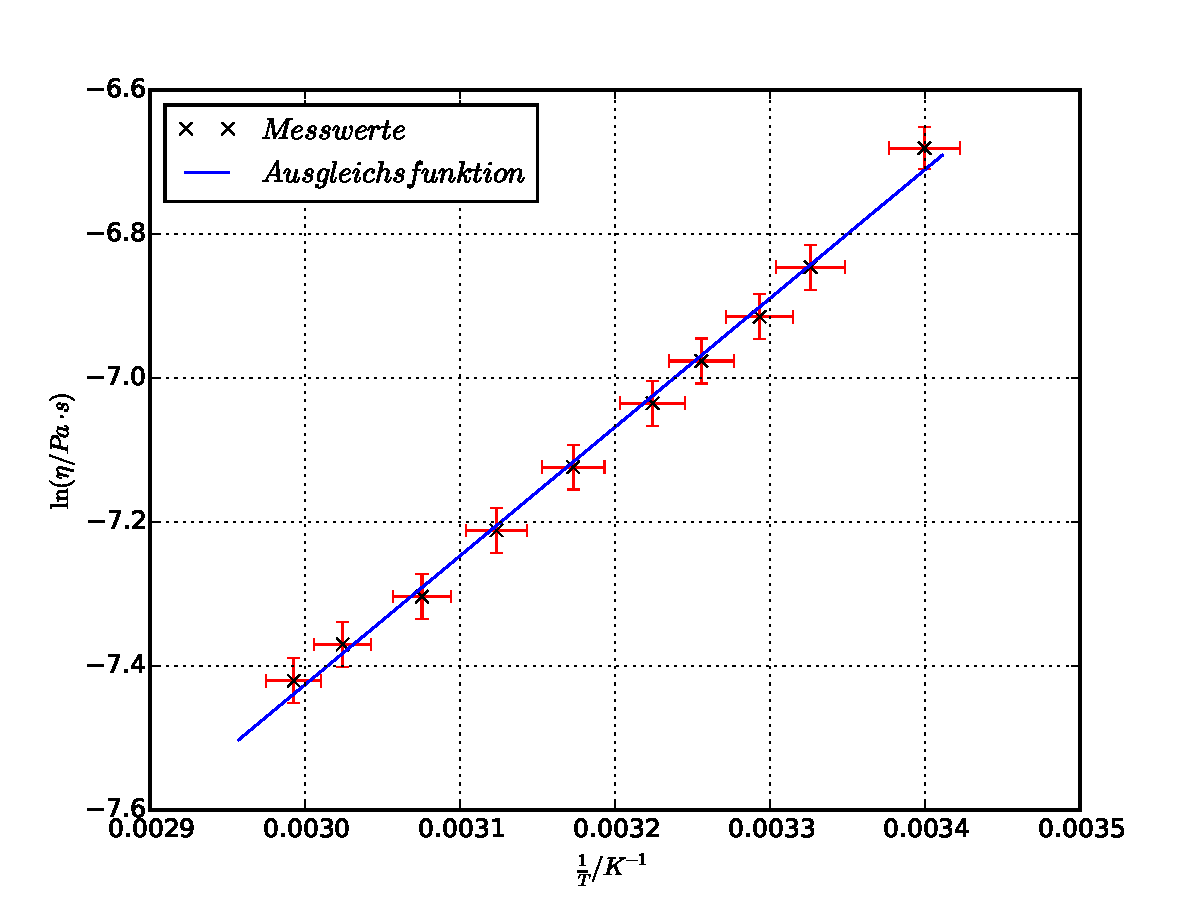
\includegraphics[width=0.7\textwidth]{plot.pdf}
  \caption{$\ln(\eta)$ gegen $1/T$ aus der Tabelle \ref{tab:temp} aufgetragen}
  \label{abb:graph}
\end{figure}
\FloatBarrier
Die Andradesche Gleichung sieht somit wie folgt aus:
\begin{align}
\ln(\eta)&=\ln\left(A\exp\left(\frac{B}{T}\right)\right).
\intertext{Diese lässt sich nun in die Graden Gleichung}
\ln(\eta)&=B\cdot\frac{1}{T}+\ln(A)
\end{align}
unformen. Somit kann nun die Lineare Regression benutzt werden, um die Kostanten B und A zu erhalten.
Aus der Linearen Regression ergibt sich für B
\begin{align}
  B=1788,46\pm39,56,\\
  \intertext{für $\ln(A)$}\\
  \ln(A)=12,79\pm0,13\\
  \intertext{und somit für A}\\
  A=(2,78\pm0,35)\cdot 10^{-6}.\\
\end{align}
\subsection{Reynoldsche Zahl}
\label{sec:rey}
Als letztes wird durch die Reynoldsche Zahl noch überprüft,
ob die hier vorkommene Strömung laminar ist.
Dafür wird die Raynoldsche Zahl mit Hilfe der Formel \eqref{eqn:rey} berechnet.
Da sich der Durchmesser der Rohre nicht bestimmen ließ, wird der Durchmesser
der größeren Kugel verwendet. Außerdem muss für die größere Kugel
nur die geringste Zeit überprüft werden, weil alle
anderen Werte durch die $1/(\eta\cdot t)$ Abhängigkeit unter diesem Wert liegen.
Für die kleinere Kugel ergibt sich
\begin{align}
Re_{\mathrm{kl}}&=97,29\pm4,22\\
\intertext{und für die größere Kugel bei der kürzesten Zeit}\\
Re_{\mathrm{gr}}&=64,59\pm2,04 .
\end{align}
laut dem Kapitel \ref{sec:theorie} handel es sich bei beiden
um eine laminare Strömung, da die Werte der beiden Reynoldschen Zahlen kleiner als $2040$ sind.
